\section{Tank Monitoring Subsystem (TMS)}
\label{sec:tms}

Il Tank Monitoring Subsystem (TMS) acquisisce il livello di
riempimento della tanica e comunica le misure al CUS tramite MQTT.


\subsection{Architettura software}
\label{subsec:tms-architecture}

Il firmware adotta un'architettura task-based basata su FreeRTOS,
con due task eseguiti su core distinti.
Il \texttt{WaterLevelTask}, assegnato al core 0, effettua
le misurazioni ed elabora il livello dell'acqua.
Il \texttt{CommunicationTask}, assegnato al core 1, gestisce
la connessione Wi-Fi e MQTT e la pubblicazione dei risultati.
Entrambi i task sono configurati con priorità 1.

La Tabella~\ref{tab:tms-tasks} riassume le responsabilità
dei due task.

\begin{table}[H]
    \centering

    \begin{tabularx}{\linewidth}{
        @{}l >{\raggedright\arraybackslash}X@{}
    }
        \toprule
        \textbf{Task} &
        \textbf{Responsabilità principale} \\
        \midrule

        \texttt{WaterLevelTask} &
        Acquisizione della distanza, verifica della validità
        e calcolo del livello di riempimento. \\

        \texttt{CommunicationTask} &
        Gestione delle connessioni Wi-Fi e MQTT,
        pubblicazione delle misure e aggiornamento
        dei LED di stato. \\

        \bottomrule
    \end{tabularx}

    \caption{Task principali del firmware TMS.}
    \label{tab:tms-tasks}
\end{table}

Lo scambio dei dati avviene tramite una coda FreeRTOS con capacità
di un elemento di tipo \texttt{WaterLevelData}.
Il task di misurazione inserisce il risultato più recente,
sostituendo un'eventuale misura non ancora prelevata;
il task di comunicazione lo legge quando può procedere
alla pubblicazione.
Questa separazione permette di continuare l'acquisizione anche
durante l'assenza della connessione, senza accumulare una sequenza
di misure precedenti da trasmettere.


\subsection{Circuito e componenti hardware}
\label{subsec:tms-hardware}

Il prototipo TMS utilizza i seguenti componenti principali:

\begin{itemize}
    \item una scheda ESP32, per l'esecuzione del firmware
    e la connessione Wi-Fi;

    \item un sensore a ultrasuoni HC-SR04, per misurare
    la distanza dalla superficie dell'acqua;

    \item un LED verde e un LED rosso, per segnalare
    lo stato della comunicazione;

    \item breadboard, cavetti e resistori per la realizzazione
    dei collegamenti.
\end{itemize}

La configurazione dei pin è centralizzata nel file
\texttt{config.h}, così da mantenere separati i collegamenti
hardware dalla logica dei task.
La Figura~\ref{fig:tms-wiring} mostra lo schema del cablaggio.

\begin{figure}[H]
    \centering

    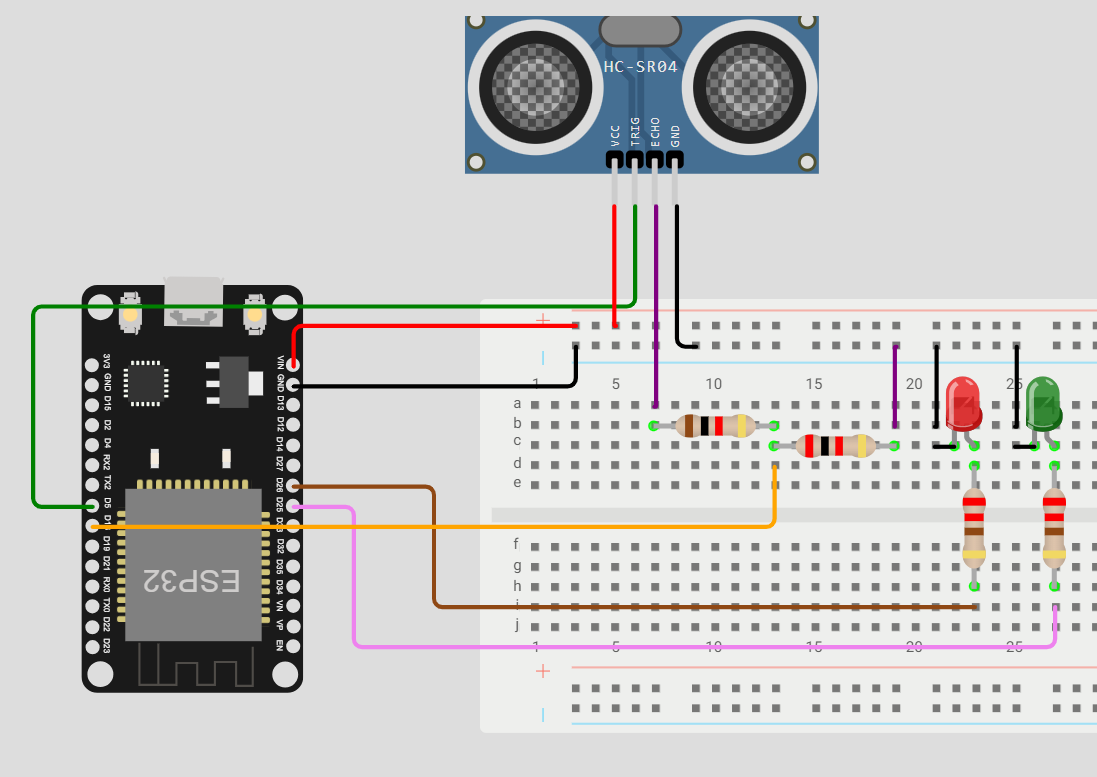
\includegraphics[
        width=0.96\linewidth
    ]{figures/tms_wiring.png}

    \caption{Cablaggio del TMS: ESP32, sonar HC-SR04
    e LED di stato.}
    \label{fig:tms-wiring}
\end{figure}

La Tabella~\ref{tab:tms-pins} riassume
i collegamenti dei segnali.

\begin{table}[H]
    \centering

    \begin{tabularx}{\linewidth}{
        @{}l >{\raggedright\arraybackslash}X@{}
    }
        \toprule
        \textbf{GPIO} & \textbf{Collegamento} \\
        \midrule

        5  & Segnale TRIG del sonar HC-SR04. \\

        18 & Segnale ECHO del sonar HC-SR04,
             attraverso il partitore resistivo. \\

        25 & LED verde di stato della comunicazione. \\

        26 & LED rosso di stato della comunicazione. \\

        \bottomrule
    \end{tabularx}

    \caption{Assegnazione dei GPIO del TMS.}
    \label{tab:tms-pins}
\end{table}

Il sonar è alimentato dalla linea a \(5\,\mathrm{V}\),
con massa comune alla scheda ESP32.
Sul segnale ECHO è presente un partitore formato da
una resistenza da \(1\,\mathrm{k}\Omega\) tra l'uscita
del sensore e il nodo collegato a GPIO18, e una resistenza
da \(2\,\mathrm{k}\Omega\) tra tale nodo e massa.
Il partitore riduce il livello alto del segnale
da circa \(5\,\mathrm{V}\) a circa \(3{,}3\,\mathrm{V}\),
rendendolo compatibile con l'ingresso della scheda.

Ciascun LED è collegato al rispettivo GPIO attraverso
una resistenza in serie da \(220\,\Omega\), che ne limita
la corrente; i catodi sono collegati a massa.


\subsection{Task del firmware}
\label{subsec:tms-tasks}


\subsubsection{CommunicationTask}
\label{subsec:tms-communication}

Il \texttt{CommunicationTask} gestisce la connessione alla rete
Wi-Fi e al broker MQTT e la pubblicazione delle misure acquisite
dal TMS.
La logica di controllo è realizzata mediante una macchina
a stati finiti, che distingue le fasi di connessione dalla
condizione di comunicazione operativa.

Gli stati principali sono:

\begin{itemize}
    \item \texttt{WIFI\_CONNECTING}: attesa della connessione
    alla rete Wi-Fi configurata;

    \item \texttt{MQTT\_CONNECTING}: tentativi di connessione
    al broker MQTT, rispettando l'intervallo di ritentativo
    configurato;

    \item \texttt{WAITING\_FIRST\_PUBLISH}: connessione MQTT
    stabilita, in attesa della prima pubblicazione riuscita;

    \item \texttt{COMMUNICATION\_OK}: almeno una pubblicazione
    è riuscita dopo la connessione MQTT corrente;
    il task continua a gestire la connessione e a pubblicare
    le nuove misure disponibili.
\end{itemize}

La Figura~\ref{fig:tms-communication-fsm} mostra
la macchina a stati del task di comunicazione.

\begin{landscape}
    \begin{figure}[p]
        \centering

        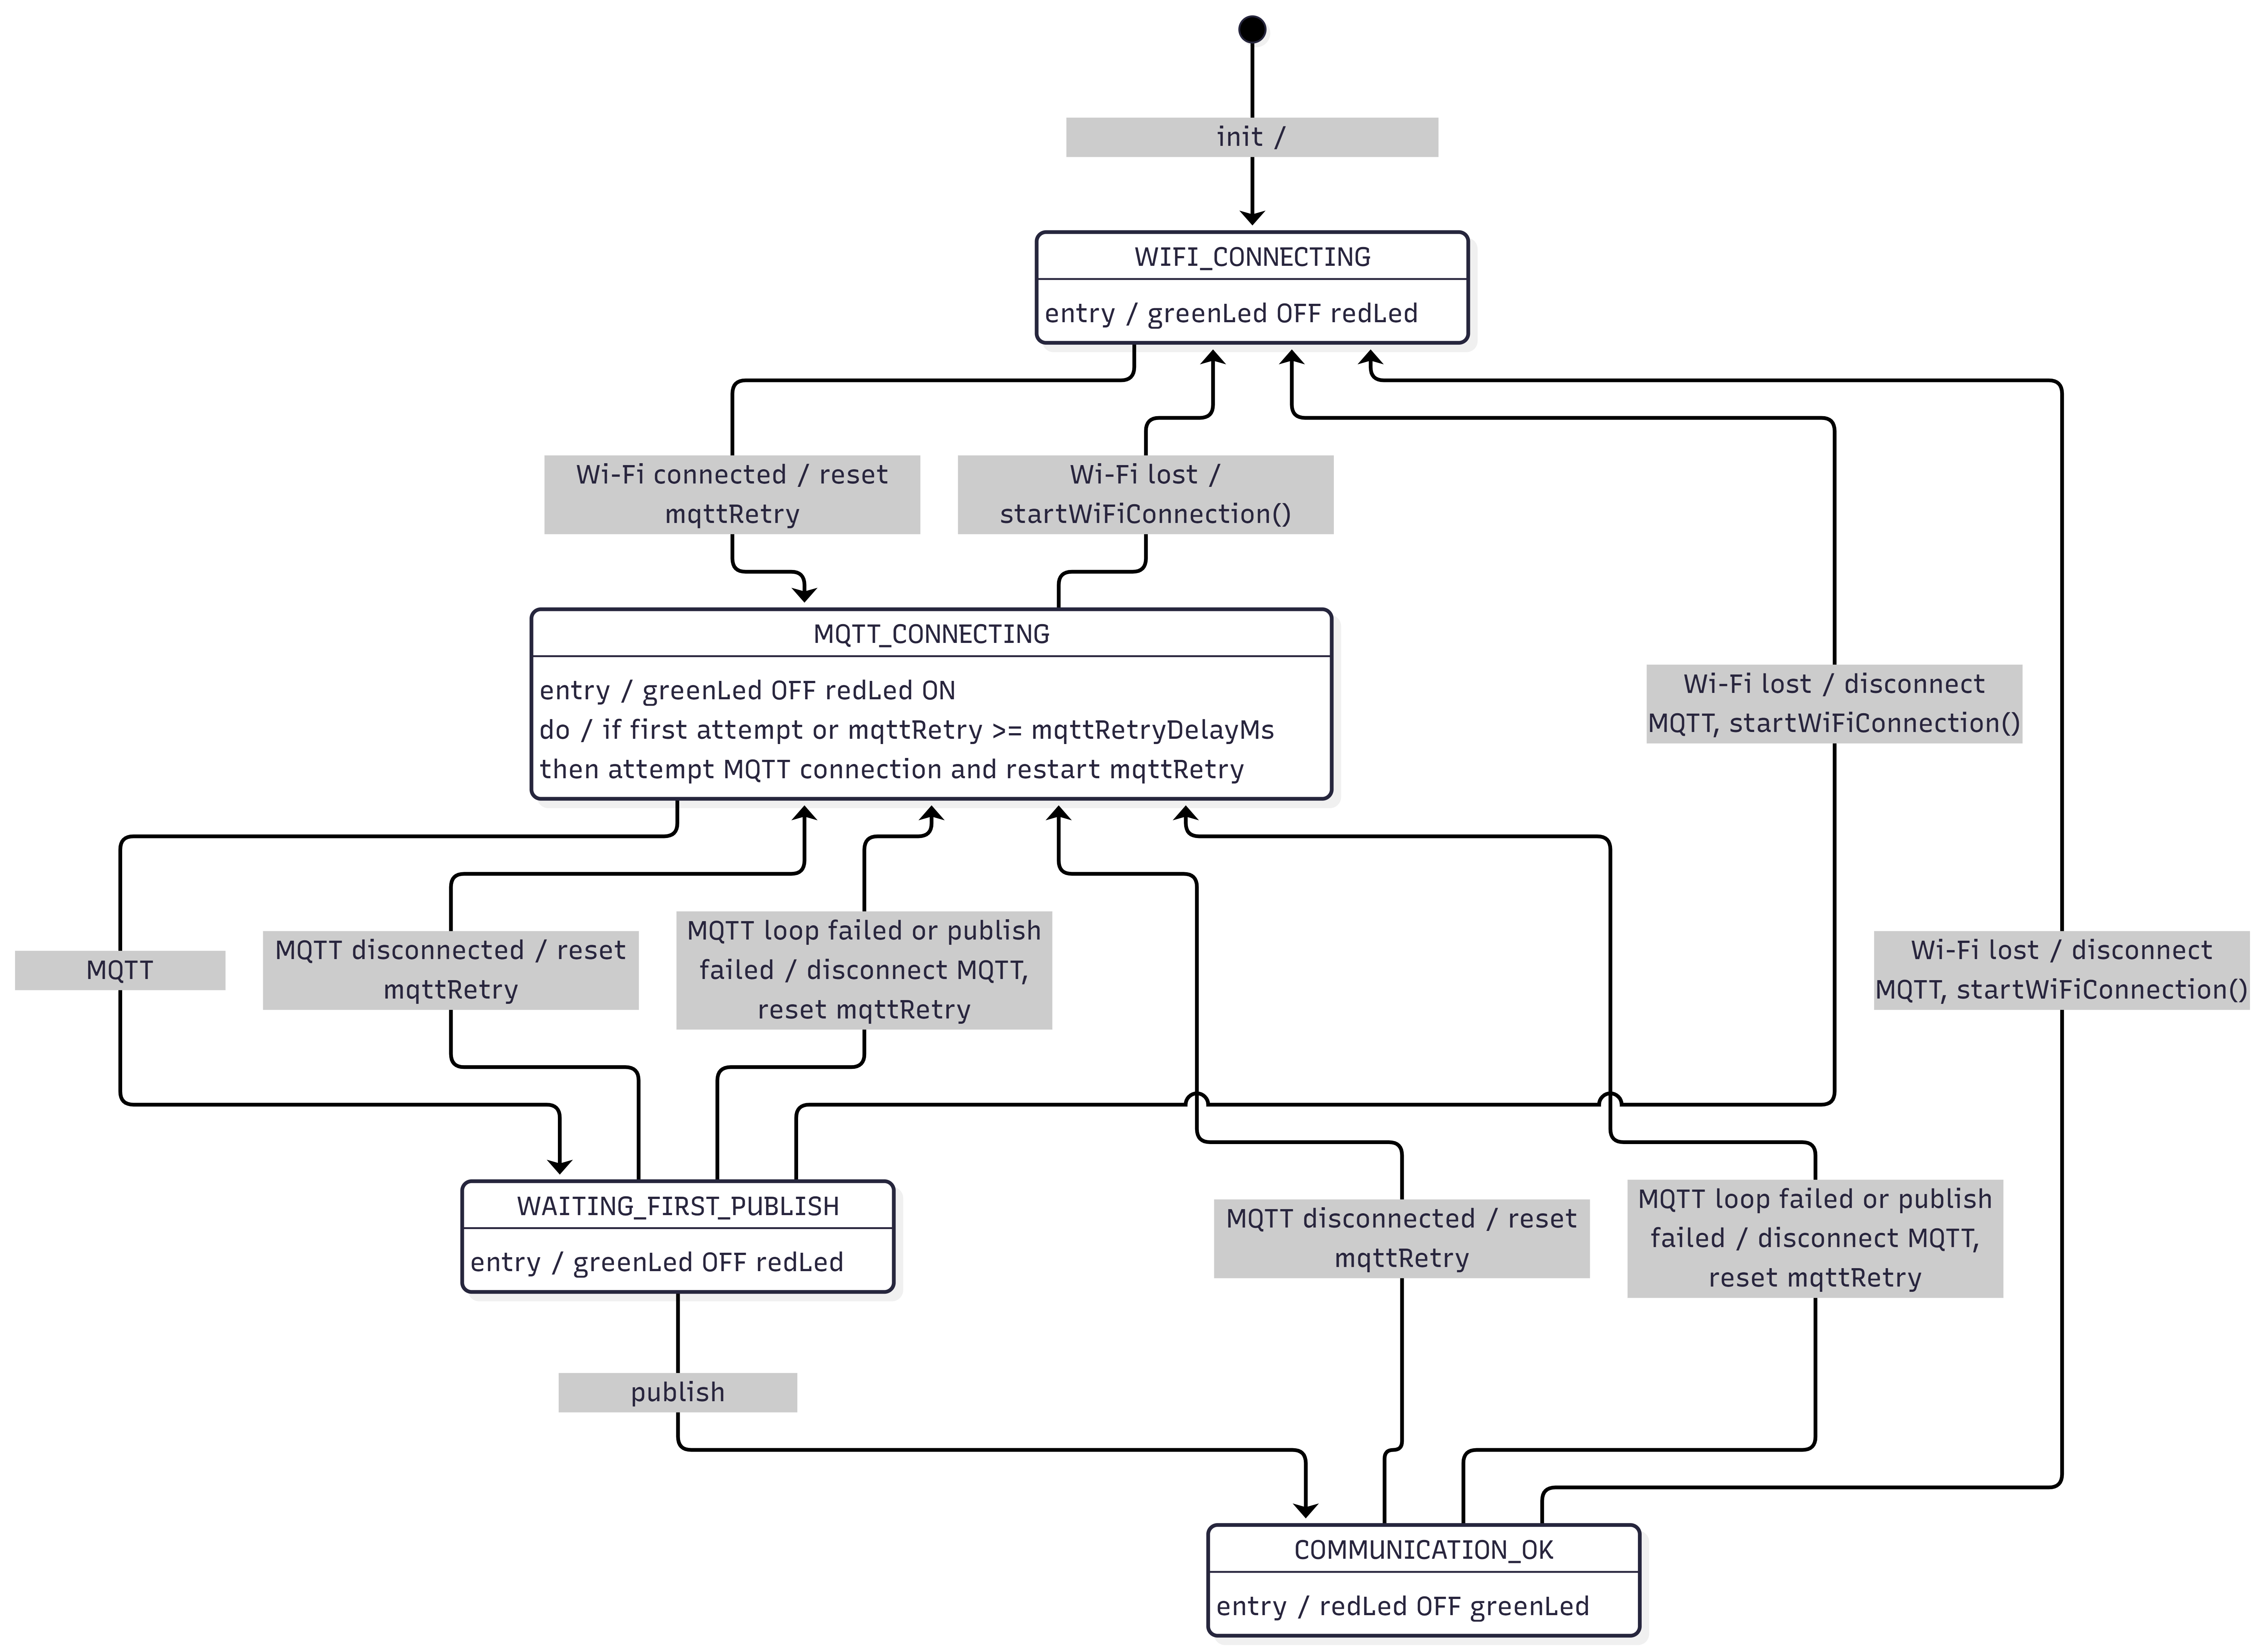
\includegraphics[
            width=\linewidth,
            height=0.90\textheight,
            keepaspectratio
        ]{figures/communication_fsm.png}

        \caption{FSM del CommunicationTask.}
        \label{fig:tms-communication-fsm}
    \end{figure}
\end{landscape}

Negli stati \texttt{WAITING\_FIRST\_PUBLISH} e
\texttt{COMMUNICATION\_OK}, il task esegue le stesse operazioni
di gestione della connessione e pubblicazione.
Richiama regolarmente \texttt{mqttClient.loop()} per mantenere
la comunicazione MQTT e, quando trova una misura nella coda,
la preleva e ne tenta la pubblicazione sul topic configurato.
Il primo esito positivo determina il passaggio a
\texttt{COMMUNICATION\_OK}; le pubblicazioni successive
proseguono nello stesso stato.

Il LED rosso rimane acceso durante la connessione Wi-Fi,
la connessione MQTT e l'attesa della prima pubblicazione riuscita.
In \texttt{COMMUNICATION\_OK} viene spento il rosso e acceso
il verde.
Quando viene rilevata una perdita della connessione,
il passaggio allo stato di riconnessione spegne il LED verde
e riaccende il LED rosso.
Il verde viene riacceso soltanto dopo una nuova pubblicazione
riuscita.
I LED rappresentano quindi lo stato della comunicazione,
indipendentemente dalla validità della misura: anche l'esito
di una lettura senza eco può essere pubblicato correttamente.

La perdita della connessione Wi-Fi determina il ritorno a
\texttt{WIFI\_CONNECTING}.
Se il Wi-Fi è disponibile ma la connessione MQTT risulta
interrotta, oppure fallisce la gestione del client o una
pubblicazione, il task passa a \texttt{MQTT\_CONNECTING}.
Il ritorno a questo stato abilita un nuovo tentativo immediato;
in caso di ulteriori fallimenti, i tentativi rispettano
l'intervallo di ritentativo configurato.

Le misure vengono pubblicate in formato JSON sul topic
definito dalla costante \texttt{MQTT\_DATA\_TOPIC}
nel file \texttt{config.h}.
Il CUS riceve i messaggi sottoscrivendo lo stesso topic.

Per una misura valida, il messaggio contiene lo stato
\texttt{OK}, il livello dell'acqua espresso in metri
nel campo \texttt{levelM} e la percentuale di riempimento
nel campo \texttt{percentage}.
Ad esempio, considerando l'altezza utile del prototipo
di \(0{,}30\,\mathrm{m}\), un livello di
\(0{,}15\,\mathrm{m}\) corrisponde a un riempimento
del \(50\%\) e produce:

\begin{verbatim}
{"status":"OK","levelM":0.150,"percentage":50.0}
\end{verbatim}

Per una lettura non valida, il messaggio contiene
soltanto l'indicazione di stato:

\begin{verbatim}
{"status":"NO_ECHO"}
\end{verbatim}

In questo caso, i campi numerici del livello e della
percentuale sono assenti.
Il CUS può quindi distinguere una lettura non valida
da una misura valida con riempimento pari allo \(0\%\).
La segnalazione viene pubblicata sullo stesso topic
utilizzato per le misure valide.


\subsubsection{WaterLevelTask}
\label{subsec:tms-water-level}

Il \texttt{WaterLevelTask} acquisisce la distanza dalla superficie
dell'acqua attraverso il sonar e calcola il livello di riempimento
della tanica.
Il periodo di acquisizione è definito nel file \texttt{config.h}
e impostato a \(2000\,\mathrm{ms}\), corrispondenti a una frequenza
di campionamento di \(0{,}5\,\mathrm{Hz}\).

Nel modello adottato, il sensore è collocato in corrispondenza
del piano che rappresenta il riempimento al \(100\%\).
Indicando con \(H\) la distanza tra il sensore e il fondo
della tanica e con \(d\) la distanza misurata dalla superficie
dell'acqua, il livello viene calcolato come:

\[
    h = H - d
\]

La percentuale di riempimento è quindi ottenuta mediante:

\[
    p = \frac{h}{H} \cdot 100
\]

La misura è considerata valida soltanto se la distanza rilevata
è compresa tra zero e \(H\).
Per le letture ammesse, il livello calcolato appartiene già
all'intervallo compreso tra zero e l'altezza della tanica,
mentre la percentuale risulta compresa tra \(0\%\) e \(100\%\).

Se la distanza è negativa, indicando l'assenza di eco,
oppure supera l'altezza configurata della tanica, il task
imposta il campo \texttt{measurementValid} a falso
e non esegue il calcolo del livello.
La lettura non valida rimane quindi distinta dalla condizione
di tanica vuota, che corrisponde invece a una misura valida
con distanza pari a \(H\).

A ogni acquisizione, il task prepara una struttura
\texttt{WaterLevelData}, contenente la validità della misura,
la distanza rilevata, il livello e la percentuale di riempimento.
La struttura viene inserita nella coda condivisa mediante
\texttt{xQueueOverwrite()}, sostituendo l'eventuale risultato
non ancora prelevato dal task di comunicazione.
Anche le letture non valide vengono inserite nella coda:
il flag di validità permette al task di comunicazione
di distinguerle dalle misure utilizzabili.

La periodicità è gestita mediante \texttt{vTaskDelayUntil()},
che riferisce i risvegli del task a scadenze periodiche,
anziché aggiungere un intervallo fisso al termine
di ogni acquisizione.


\subsection{Scelte progettuali e gestione degli errori}
\label{subsec:tms-design-choices}

Le principali scelte progettuali riguardano la continuità
dell'acquisizione, la gestione delle misure e la configurazione
del prototipo:

\begin{itemize}
    \item \textbf{Separazione tra acquisizione e comunicazione.}
    Le due attività sono affidate a task distinti, così che
    l'attesa della connessione Wi-Fi o MQTT non interrompa
    il campionamento del livello dell'acqua.

    \item \textbf{Priorità alla misura più recente.}
    La coda condivisa contiene un solo elemento e viene
    aggiornata mediante sovrascrittura.
    Questa scelta privilegia la disponibilità dello stato
    corrente della tanica, evitando l'accumulo di misure
    da trasmettere dopo un'interruzione della connessione.

    \item \textbf{Distinzione tra lettura non valida
    e tanica vuota.}
    La validità viene rappresentata esplicitamente
    nella struttura della misura.
    Una lettura non utilizzabile viene comunicata mediante
    lo stato \texttt{NO\_ECHO}, mentre una tanica vuota
    corrisponde a una misura valida con livello pari a zero.

    \item \textbf{Configurazione centralizzata.}
    I pin, i parametri di rete, i periodi dei task
    e l'altezza utile della tanica sono raccolti
    nel file \texttt{config.h}.
    Il valore dell'altezza deve corrispondere alla distanza
    effettiva tra il sensore e il fondo, coerentemente
    con il modello utilizzato per il calcolo del livello.
\end{itemize}

Le interruzioni della connessione vengono gestite
dalla macchina a stati del \texttt{CommunicationTask},
che effettua nuovi tentativi di connessione senza richiedere
il riavvio della scheda.
Il LED rosso segnala la condizione di comunicazione
non operativa durante il recupero.

Gli errori di inizializzazione vengono invece rilevati
controllando il risultato della creazione della coda
e dei task FreeRTOS.
In caso di fallimento, viene stampato un messaggio diagnostico
sulla porta seriale e viene sospeso il task Arduino
che esegue \texttt{setup()}, mediante
\texttt{vTaskSuspend(nullptr)}.
La sospensione impedisce di proseguire l'inizializzazione
con risorse mancanti e riguarda soltanto il task chiamante:
gli eventuali task già creati rimangono attivi.


\subsection{Test, criticità e taratura}
\label{subsec:tms-tests}
\paragraph{Allestimento e verifica delle misure.}

Le prove del TMS sono state effettuate utilizzando una
scatolina in polimero di forma geometrica regolare come
bersaglio del sonar.
Variando la distanza tra il sensore e l'oggetto sono stati
simulati diversi livelli di riempimento della tanica.

L'altezza utile è stata configurata a
\(0{,}30\,\mathrm{m}\), corrispondenti alla lunghezza
del righello utilizzato come riferimento.
La distanza rilevata dal sonar è stata confrontata
con quella misurata mediante il righello, posizionando
la scatolina a distanze differenti dal sensore.
Le letture sono risultate approssimativamente
corrispondenti alle distanze di riferimento,
fornendo una verifica qualitativa dell'acquisizione
nella configurazione utilizzata.

È stata verificata anche la coerenza tra il livello
espresso in metri e la percentuale di riempimento,
rispetto all'altezza configurata.
Con un'altezza utile di \(0{,}30\,\mathrm{m}\),
un livello di \(0{,}15\,\mathrm{m}\) corrisponde
a un riempimento del \(50\%\).

\paragraph{Gestione delle letture non valide.}

Durante le prove preliminari con la mano come bersaglio
sono state osservate letture non valide, segnalate come
\texttt{NO\_ECHO}.
È stato quindi utilizzato un oggetto di forma regolare
per proseguire le verifiche.

È stata controllata anche la gestione delle distanze
superiori all'altezza configurata, collocando il bersaglio
oltre i \(30\,\mathrm{cm}\).
La lettura è stata correttamente classificata come
non valida e comunicata mediante lo stato
\texttt{NO\_ECHO}.
Per le letture non valide è stata verificata la gestione
sul CUS, che ha riconosciuto la segnalazione e restituito
\texttt{null} per la misura non disponibile.
Il comportamento osservato distingue quindi una misura
non utilizzabile da una misura valida con livello
pari a zero.

\paragraph{Avvio e recupero della comunicazione.}

È stata verificata la segnalazione luminosa durante
l'avvio del TMS e dopo un riavvio manuale mediante
il pulsante RESET della scheda.
In entrambi i casi è stata osservata l'accensione
iniziale del LED rosso, seguita dal passaggio al verde
al ripristino della comunicazione.
Questa sequenza è coerente con la macchina a stati,
che abilita il verde dopo la prima pubblicazione MQTT
riuscita.

È stata inoltre verificata la gestione della perdita
della connessione Wi-Fi durante il funzionamento,
interrompendo temporaneamente la rete e mantenendo
la scheda accesa.
Al ripristino della rete, il TMS ha ristabilito
automaticamente la comunicazione, tornando alla
condizione operativa segnalata dal LED verde.
Il recupero è avvenuto senza richiedere un riavvio
manuale della scheda.